\chapter{Introduction}\label{ch1:Intro}

%Try to describe the mechanical response of materials from first principles is an intelectual exercise that I found to be interesting enough to dedicate 2 years of my time and maybe more.

% About this thesis

The aim of this work is to describe the mechanical response of hydrogels from first principles. 
Conducted over a two-year period, the research lays the foundation for further investigations, such as the design of synthesis methods for hydrogels with tailored mechanical properties. 
The proposed methodology relies on prior research in which the polymeric network of PNIPAM microgels was replicated using molecular dynamics with patchy particles.

A review of the literature reveals that hydrogels have a wide range of applications.
However, the precise origin of the mechanical response in hydrogels remains a topic of debate.
Thus, the main the key objective of this thesis is to explore a computational methodology capable of identifying parameters that can model the main properties of the polymeric network. 
These parameters can then be coupled into a constitutive relations to predict the mechanical response of a simplified polymeric network.
To that end, we have established the following specific objectives:
\begin{itemize}
    \item Replicate the existing numerical protocol.
    \item Adapt the protocol to create a more general network.
    \item Apply controlled shear deformations.
    \item Characterize the network before and after shear.
    \item Analyze the strain-stress curves of the material under different shear conditions and different network parameters.
\end{itemize}
The analysis is expected to help selective one or more parameters that can later be incorporated into a constitutive equation.
It is important to clarify that the explicit formulation of such an equation is not within the scope of this thesis. 
The objective is to identify a relation between the network characteristics and its mechanical response.

The following section, explores the applications of hydrogels identified in the literature review, followed by a discussion of their characteristic mechanical responses.
The subsequent theoretical framework chapter begins by explaining how to quantify the properties of the material and how to apply numerical simulations to analyze the system.
The last part of this work covers the analysis of the numerical results and the conclusions.

\section{About Hydrogels}

While the numerical protocol was initially developed for a specific polymeric network, it was modified to represent a simplified case that resembles a broader group of polymeric networks.
These polymeric networks are collectively referred to as hydrogels.
Hydrogels are composed primarily of hydrophilic monomers, which are biocompatible, making them suitable for medical applications.
In general terms, hydrogels exhibit viscoelastic and viscoplastic mechanical responses.
The material's viscoelasticity response makes it suitable for use in shock absorption, vibration damping, and biological tissue mimicry.
Meanwhile, the viscoplasticity response makes the material suitable for energy dissipation.
First, we will explore various applications of this material.
Then, we will provide a brief introduction to viscoelasticity and viscoplasticity responses.

\subsection{Applications}

The selection of applications is guided by three key factors. 
First, considering the imminent threat that climate change poses to the global environment, investigating environmentally relevant applications is a priority.
Second, to align with the institution's strategic research interests in biomedical applications.
Lastly, from prior academic experience in smart materials, some examples from this sectors where included.

%\paragraph{Environmental applications} 
By the chemical structure, hydrogels can effectively remove a wide range of toxic compounds, such as heavy metals, organic pollutants and pathogens from aqueous environments.
Reference~\citep{cinfrigniniGoldRushDesigning2024} explores an easy-to-make poly(acrylamide-co-acrylic acid) hydrogels as adsorbents for gold recovery from industrial wastewater containing other precious metals.
This review~\citep{randoFunctionalBioBasedPolymeric2024} investigates the emerging topic of stimuli-responsive smart hydrogels, underscoring their potential in both adsorption and detection of water pollutants.
On this other review~\citep{darbanHydrogelBasedAdsorbentMaterial2022a} explains the synthesis and adsorption mechanicsms in detail with the understanding of the regeneration, recovery, and reuse of hydrogel-based adsorbent materials.
Finally in the reference~\citep{songSynthesisHydrogelsTheir2022} different synthetic strategies, crosslinking methods and their corresponding limitations and outstanding contributions of applications in the fields of removing environmental pollutants are reviewed to further provide a prospective view of their applications in water resources sustainability.

%\paragraph{Medical applications} 
Hydrogels have garnered significant attention as versatile materials for biomedical applications due to their high water content, biocompatibility, and tunable properties. 
They mimic natural tissue environments, enhancing cell viability and function.
Reference~\citep{wuAdvancementsHydrogelsCorneal2024} they discuss the fundamentals of hydrogels, emphasizing their relevance to corneal tissue engineering, and explore various types of hydrogels, including stimuli-responsive variants.
Reference~\citep{kaurHydrogelsPotentialBiomaterial2024} highlight some of the recent interesting applications of bioactive hydrogels in the field of antibacterial wound healing, oral delivery of drugs, cancer immunotherapy, tissue regeneration, and similar potential biomedical aspects.
Finally, reference~\citep{thummaIntroductionClassificationApplications2025} presents a thorough investigation of the synthesis and medicinal uses of different naturally occurring and synthetic hydrogels, for cancer therapy, mainly via 3D modeling and printing.

%\paragraph{Smart materials} 
Stimuli-responsive hydrogels are emerging as smart materials due to their tunable chemical and physical properties in response to various stimuli such as pH, temperature, chemicals, pressure, electrical or light. 
In~\citep{bishnoiCellulosebasedSmartMaterials2024}, we have discussed the role and overview of cellulose‐based hydrogels in elements of energy storage systems.
According to~\citep{zhaoIntelligentHydrogelActuators2021} near infrared laser driven intelligent hydrogel actuator systems with a high response rate were prepared via three-dimensional printing and hydrothermal synthesis.
As reported in~\citep{shomePhotoresponsiveSmartHydrogels2024}, basic mechanisms responsible for photo-responsiveness in hydrogels along with their potential applications are discussed.
Finally, reference~\citep{duttaSmartMaterialsFlexible2024}, they discuss the state-of-the-art applications of hydrogels in flexible electronics, such as energy storage, touch panels, memristor devices, and sensors like temperature, gas, humidity, chemical, strain, and textile sensors, and the latest synthesis methods of hydrogels.

% Clousure/transition paragraph
Several of these applications are illustrated in Figure~\ref{fig:applications} and discussed in \citep{petelinsekToughHydrogelsLoadBearing2024}. 
Although there is experimental data on potential applications, a fundamental explanation of the molecular mechanisms that enable this diversity based on first principles is still lacking. 
The intention of this work is therefore to validate a simulation methodology with the ultimate goal of providing a basis for optimising their formulation. 
Having established this context, we now explore the mechanical properties that enable such a wide range of applications.

\begin{figure}[ht!]
    \centering
    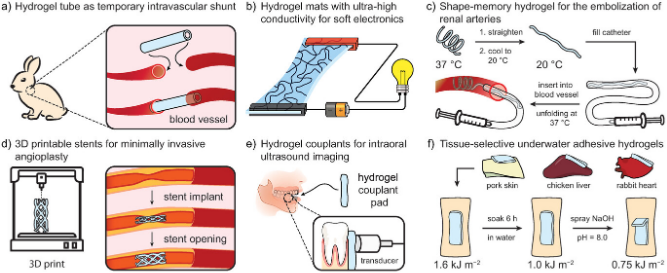
\includegraphics[width=12cm]{figs/applications.png}
    \caption{Examples of tough hydrogels applied in the areas of a) tissue engineering, b) soft electronics, c) shape memory materials, d) 3D printing, e) biomedical devices, and f) adhesives. 
    It is worth noting that the majority of the highlighted examples have biomedical applications.\citep{petelinsekToughHydrogelsLoadBearing2024}.}\label{fig:applications}
\end{figure}

\subsection{Mechanical response}

The origin of the mechanical properties of hydrogels from first principles remains incompletely understood due to the complex multi-scale nature of these materials\citep{senffTemperatureSensitiveMicrogel1999}.
Hydrogels consist of heterogeneous, often disordered polymer networks swollen with water, where molecular interactions (covalent bonds, physical crosslinks, entanglements, and solvent–polymer interactions) collectively determine macroscopic elasticity and viscoelasticity. 
Accurately bridging atomic-scale forces and chemical bond dynamics to bulk mechanical behavior involves coupling nonlinear polymer physics, solvent effects, and dynamic crosslink kinetics. 
Which presents a significant challenge to current theoretical and computational models. 

Viscoelastic materials exhibit a mechanical response that lies between elastic and plastic deformation.
Hydrogels, initially respond elastically to a force and then undergo continuous viscous deformation.
This continuous viscous deformation is known as ``creep''.
Furthermore, when subjected to a constant strain, viscoelastic materials experience ``stress relaxation'', whereby stress decreases over time after the yield point.

When a hydrogel is deformed, the bonds, intermolecular distances, molecular conformation and chain orientation are modified accordingly.
Furthermore, any molecular event resulting in energy dissipation contributes to viscoelasticity, given the direct correlation between viscosity and energy dissipation.
One such factor is the polymer molecular weight, which affects the movement of entangled polymers.
Another factor that promotes molecular mobility is the interconnectivity and cohesion of the network.
These processes enable network flow under an applied force, thereby facilitating viscoelasticity.

Another factor influencing viscoelastic behaviour is the strength of the crosslinking mechanisms in the network.
In the case of weak crosslink mechanisms, stress relaxation is observed; however, in strongly crosslinked hydrogels, this process is prevented. 
This is due to the fact that weak bonds permit the release of energy and the separation of elements under force, thereby facilitating network relaxation or creep.
Furthermore, weak bonds are capable of responding to force by dissociating and rebinding, which can result in plastic or permanent deformations.
This is in contrast to strong crosslink mechanisms, which prevent the network from flowing and dissipating energy, thereby promoting the material's predominantly elastic properties.
It is widely accepted that permanent cross-links are responsible for the elastic properties of the material, while dynamic cross-links regulate energy dissipation.

Finally, the water content has a significant impact on the viscoelasticity of the hydrogels.
Applying pressure to the hydrogels causes water to flow in or out of the network, resulting in a time-dependent response due to changes in volume. This leads to strand extension and therefore firmness enhancement.
This phenomenon is known as poroelasticity. 
It is important to note that these changes result in viscous dissipation, which in turn impacts the viscoelastic properties\citep{sheikoArchitecturalCodeRubber2019,courbotRoleExtracellularMatrix2025}.

The previous characteristics are quantify by the strain-stress relation.
On figure~\ref{fig:mechresponse0-a} it is a graphical resume of the strain-stress relation for an elastics, plastic and viscoelastic material.
When a constant force (stress) is applied in an elastic material, the material deformes instantly and mantains that deformation until the load is remove, at wich point it returns to its original shape (panel a.1).
However, when this constant force applied in a viscous material, the deformation is no longer instantaneous, instead, it undergoes continuous deformation and when the applied force is removed, the material stays in the deformed shape (panel a.2).
Therefore, when a viscoelastic material is deformed, it displays an initial immediate response to the force, followed by an increase in the defomation over time, then, when the force it is remove, the material recovers its original shape (panel a.3).

\begin{figure}[ht!]
    \centering
    \centering
    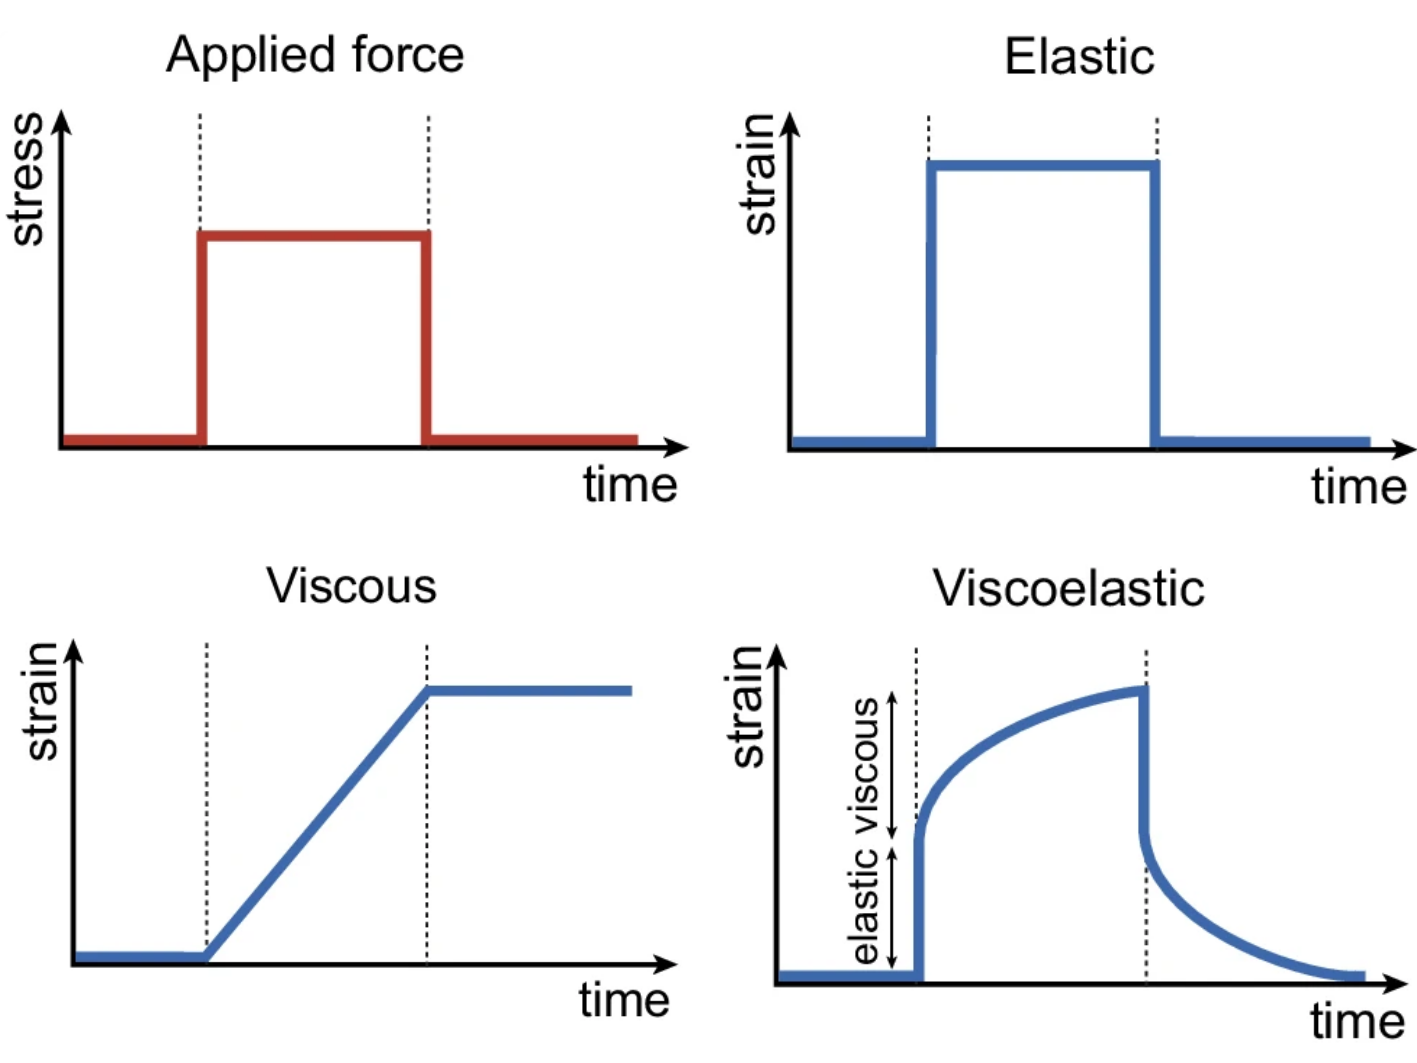
\includegraphics[width=10cm]{figs/mechResponse/viscoElasticResponse-1.png}
    \caption{Deformation at constant stress in an elastic (left), viscous (middle) and viscoelastic materials (right). Figure retrieve from\citep{courbotRoleExtracellularMatrix2025}}\label{fig:mechresponse0-a}
\end{figure}

Delveving into more specific viscoelastic properties, figure~\ref{fig:mechresponse0-b} shows the creep and stress relaxation strain-stress relation for viscoelastic materials.
When the viscoelastic material is under a constant force, the material starts to elastically deform.
The more viscoelasitc the material is, the more it deformes over time under the load.
Once the force it is removed, the deformation starts to undo.
On the other hand, when a constant deformation it is applied to a viscoelastic material, the stress increases like an elastic material, however, the stress starts to reduce over the applied deformation.
The more viscoelastic is the material, the faster the stress decreases. 
Once the deformation it is removed, the stress goes to zero.

\begin{figure}[ht!]
    \centering
    \centering
    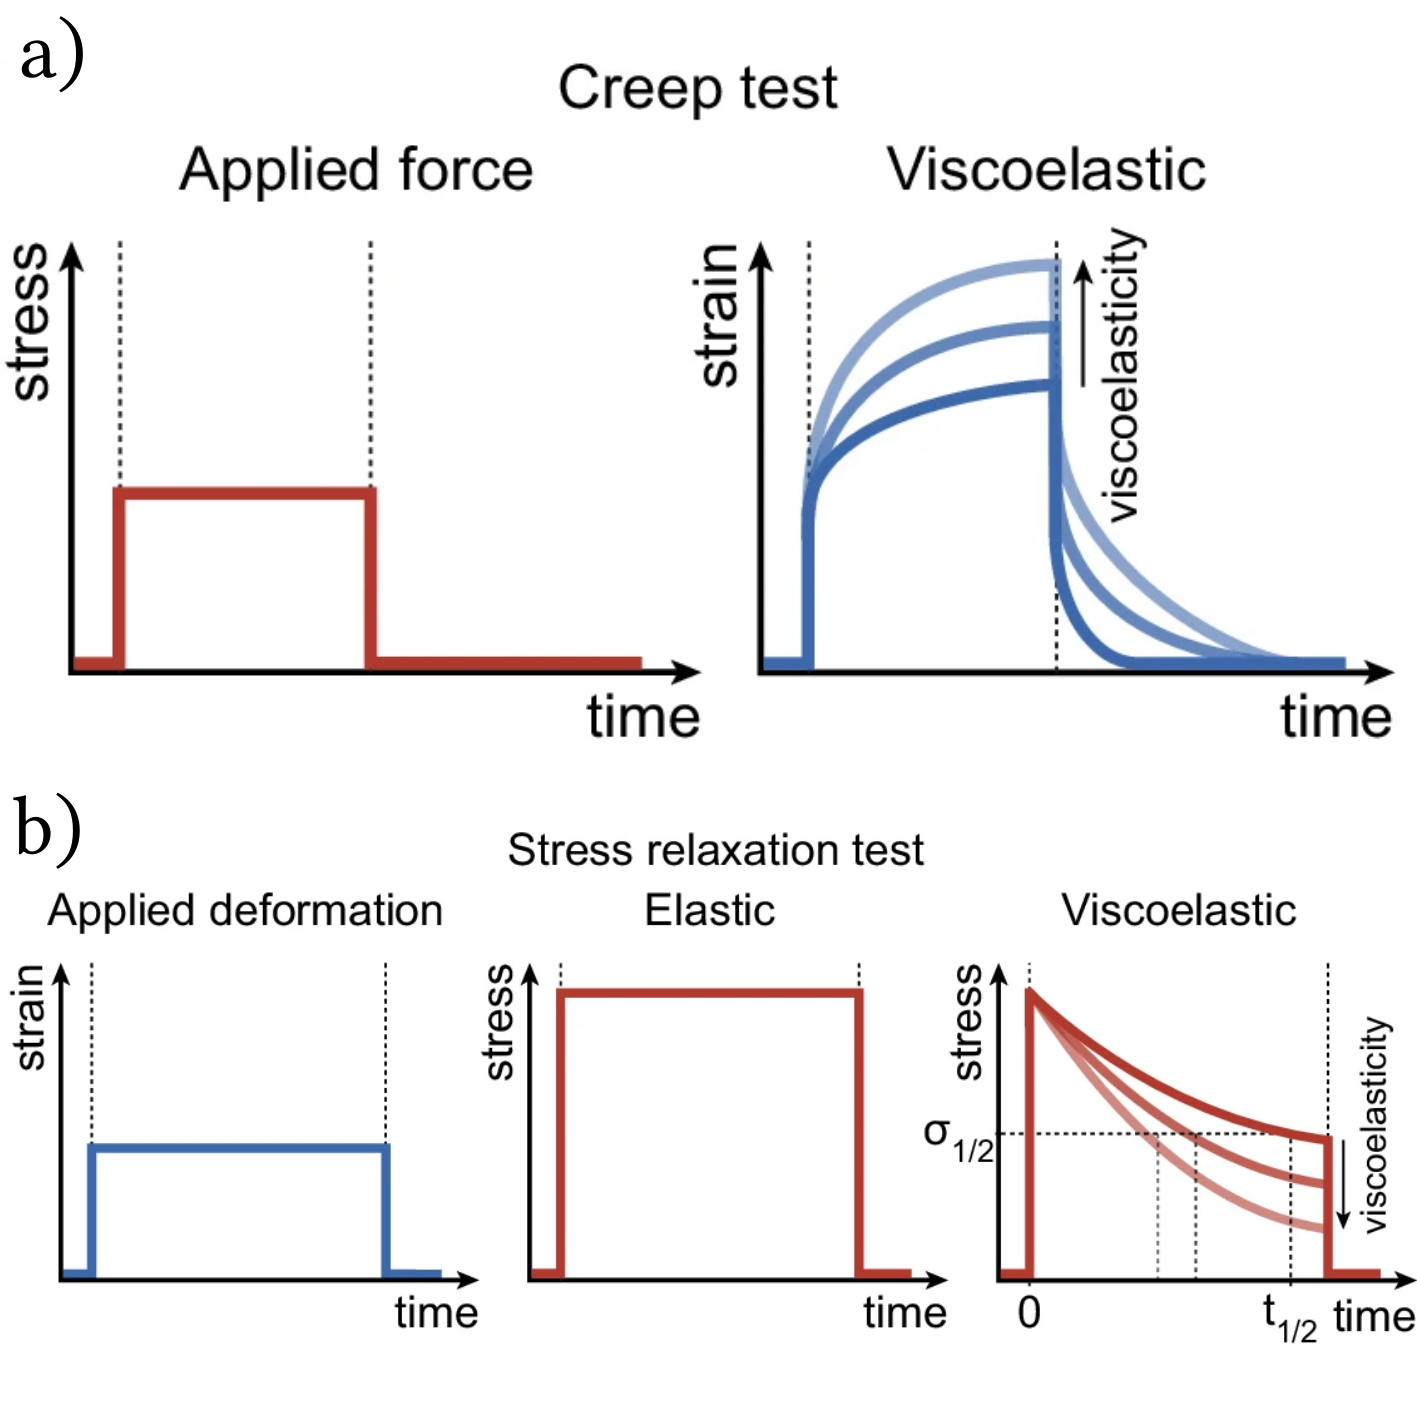
\includegraphics[width=10cm]{figs/mechResponse/viscoElasticResponse-2.png}
    \caption{Deformation at constant stress in a viscoelastic material.
        Creep response at the left and the stress relaxation behaviour at the right.
        Figure retrieve from\citep{courbotRoleExtracellularMatrix2025}}\label{fig:mechresponse0-b}
\end{figure}

Finally, it is important to notice that when the deformation goes beyond the plastic limit, the material has a plastic deformation.
In figure~\ref{fig:mechresponse0-c} it is shown the creep response of the viescoelastic material under constant force, and when the stress is removed, the deformation remains.

\begin{figure}[ht!]
    \centering
    \centering
    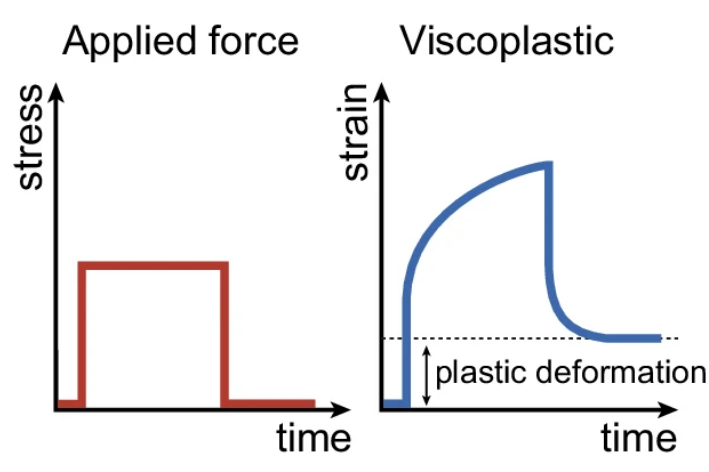
\includegraphics[width=10cm]{figs/mechResponse/viscoElasticResponse-3.png}
    \caption{Creep response of viscoelastic materials. 
        Figure retrieve from\citep{courbotRoleExtracellularMatrix2025}}\label{fig:mechresponse0-c}
\end{figure}

In this regard, the key point for the thesis is to explore how we can use molecular dynamics to determine the extent to which the mechanical response of hydrogels can be explained by the topological features of the polymeric networks.
In addition, elucidate a methodology to quantify the influence of the cross-linker concentration and dynamics in the response.
In the following chapter, we will explore the mathematical tools that enable us to quantify this relationship.
Furthermore, we will provide a comprehensive explanation of how these relationships can be simulated using molecular dynamics. 
We will also discuss the correlation between numerical simulations and experimental results.


%\paragraph{Clousure paragraph}

